\chapter{Studio del campionamento}
\label{ch:studio}

Nei capitoli precedenti sono stati introdotti gli strumenti teorici necessari a campionare una distribuzione di Boltzmann: il campionamento markoviano locale via Metropolis-Hastings (Sez.~\ref{sec:mcmc}), i normalizing flow (Capitolo~\ref{ch:nf}) e da quest'ultimo è stato derivato anche uno schema ibrido, il Flow-MCMC. Questi tre metodi condividono l'obiettivo ma differiscono radicalmente nella strategia: MCMC locale esplora lo spazio delle configurazioni muovendosi solo nell'intorno immediato dello stato corrente; il normalizing flow genera campioni indipendenti, pagando il prezzo di un addestramento preliminare e di un possibile disallineamento tra la distribuzione appresa e quella target; il Flow-MCMC combina le due prospettive mantenendo convergenza asintotica e campionamento globale. La domanda naturale è se questa differenza di strategia si traduca in una differenza pratica misurabile nella qualità del campionamento.

Per rispondere si è scelto, come sistema di test, un potenziale a doppio pozzo lungo una coordinata, descritto in Sezione~\ref{sec:potenziale_dw}. Questo sistema ha la minima richiesta di multimodalità, essendo bimodale, e dunque è il caso più semplice in cui ci si aspetta che le strategie locali di campionamento, come Metropolis-Hastings standard, entrino in difficoltà; alla coordinata bimodale si possono affiancare ulteriori dimensioni puramente armoniche, che non aggiungono multimodalità ma permettono di studiare l'effetto della dimensionalità complessiva del sistema sulla qualità del campionamento.

Lo studio si articola in due parti. Nella Sezione~\ref{sec:limiti_mcmc} si studia il comportamento termodinamico del sistema utilizzando solo MCMC locale al variare del numero di dimensioni del sistema, mantenendo sempre la prima variabile nel doppio pozzo e aggiungendo un numero crescente di dimensioni armoniche,quantificando il fallimento attraverso l'acceptance rate, il tempo di autocorrelazione integrato. La Sezione~\ref{sec:confronto_metodi} confronta invece i tre metodi --- MCMC locale, NF con re-weighting e Flow-MCMC --- a dimensione fissata $D=3$ (una variabile in potenziale doppio pozzo e due armoniche), sia al variare della temperatura sia al variare del numero di campioni utilizzati. 

\section{Il potenziale doppio pozzo}
\label{sec:potenziale_dw}

Il potenziale doppio pozzo è definito da
\begin{equation}
    V_{\text{dw}}(x) = \frac{a}{b^4}\left(x^2 - b\right)^2,
\end{equation}
e viene scelto agente lungo una sola coordinata, mentre le rimanenti $D-1$ direzioni sono trattate come oscillatori armonici disaccoppiati. Il potenziale totale, per $\mathbf{x} = (x_1, \mathbf{x}_\perp) \in
\mathbb{R}^D$, è quindi
\begin{equation}
    V(\mathbf{x}) = \underbrace{\frac{a}{b^4}\left(x_1^2 - b\right)^2}_{V_{\text{dw}}(x_1)}
    \;+\; \underbrace{\frac{1}{2}\sum_{i=2}^{D} x_i^2}_{V_{\text{arm}}(\mathbf{x}_\perp)},
    \qquad a, b > 0.
    \label{eq:double_well_potential}
\end{equation}
La coordinata $x_1$ è detta "lenta",poichè vede la struttura a doppia buca, mentre $\mathbf{x}_\perp = (x_2,\dots,x_D)$ raccoglie le direzioni "veloci", puramente armoniche e prive di barriere.
Il termine $V_{\text{dw}}(x_1)$ ha due minimi in $x_1 = \pm\sqrt{b}$, separati da una barriera in $x_1 = 0$ di altezza
%
\begin{equation}
    \Delta V = V_{\text{dw}}(0) = \frac{a}{b^2}.
    \label{eq:barrier_height}
\end{equation}
%
Il potenziale è pari su ogni variabile, $V(-x_i) = V(x_i)$, e la distribuzione di Boltzmann associata eredita la stessa simmetria, $p(-x_i) = p(x_i)$. Una conseguenza diretta è il segno medio $\langle \operatorname{sgn}(x_1) \rangle$ è nullo, infatti:
\begin{equation}
    \langle \operatorname{sgn}(x_1) \rangle
    = \int_{\mathbb{R}^D} p(\mathbf{x}) \, \operatorname{sgn}(x_1) \, d\mathbf{x}.
\end{equation}
Operando il cambio di variabile $x_1 \to -x_1$ (a $\mathbf{x}_\perp$ fissato,
con $d\mathbf{x}$ invariante) si ottiene
\begin{equation}
    \langle \operatorname{sgn}(x_1) \rangle
    = \int_{\mathbb{R}^D} p(-x_1, \mathbf{x}_\perp) \, \operatorname{sgn}(-x_1) \, d\mathbf{x}
    = -\int_{\mathbb{R}^D} p(x_1, \mathbf{x}_\perp) \, \operatorname{sgn}(x_1) \, d\mathbf{x}
\end{equation}
dove nel secondo passaggio si è usata la parità di $p$ e la disparità di $\operatorname{sgn}$, $\operatorname{sgn}(-x_1) = -\operatorname{sgn}(x_1)$. Nell'ultimo passaggio possiamo risostituire la definizione di segno medio e da $\langle \operatorname{sgn}(x_1) \rangle = -\langle \operatorname{sgn}(x_1) \rangle$ segue immediatamente
\begin{equation}
    \langle \operatorname{sgn}(x_1) \rangle = 0.
\end{equation}

Nella simulazione si è fissato $a = 0.1$~eV e $b = 1.0$ (in unità della coordinata $x_1$), da cui, per l'Eq.~\eqref{eq:barrier_height}, una barriera $\Delta V = 0.1$~eV, con minimi in $x_1 = \pm 1$.

Il parametro rilevante per il grado di difficoltà del campionamento è il rapporto adimensionale $\Delta V / (k_B T)$ tra l'altezza della barriera e l'energia termica disponibile. Le temperature esplorate sono all'interno dell'intervallo $T \in [100, 1100]$~K e dunque il rapporto avrà un valore minimo e un valore massimo:
%
\begin{equation}
    \frac{\Delta V}{k_B T}\bigg|_{T = 1100~\text{K}} \approx 1.05,
    \qquad
    \frac{\Delta V}{k_B T}\bigg|_{T = 100~\text{K}} \approx 11.6.
\end{equation}
%
Alle temperature più alte la barriera è dell'ordine dell'energia termica: la catena di Markov con proposte locali la attraversa facilmente. Alle temperature più basse la barriera diventa fortemente soppressa in probabilità ($e^{-\Delta V/k_BT} \sim e^{-11.6} \approx 9\times10^{-6}$), è in questo regime che ci si aspetta il fallimento del campionamento locale, e il vantaggio dei metodi basati su normalizing flow.

Il termine armonico $V_{\text{arm}}(\mathbf{x}_\perp)$ è disaccoppiato da $x_1$ e, per equipartizione, contribuisce esattamente $\tfrac{1}{2}(D-1)k_BT$ all'energia media: la sua funzione è puramente quella di aggiungere gradi di libertà al sistema senza aggiungere barriere energetiche e quindi senza aggiungere altre variabili multimodali. Questa separabilità rende inoltre disponibile un riferimento per l'energia media, ottenuto per quadratura numerica 1D sulla sola coordinata $x_1$ e sommando il
contributo armonico in forma chiusa; questo valore $\langle E \rangle_{\text{esatto}}(T)$ verrà usato come riferimento nei confronti al variare di $N$ in Sezione~\ref{sec:confronto_metodi}. 

\section{Limiti di Markov Chain Monte Carlo}
\label{sec:limiti_mcmc}
\subsection{Dettagli implementativi}
\begin{figure}[H]
    \centering
    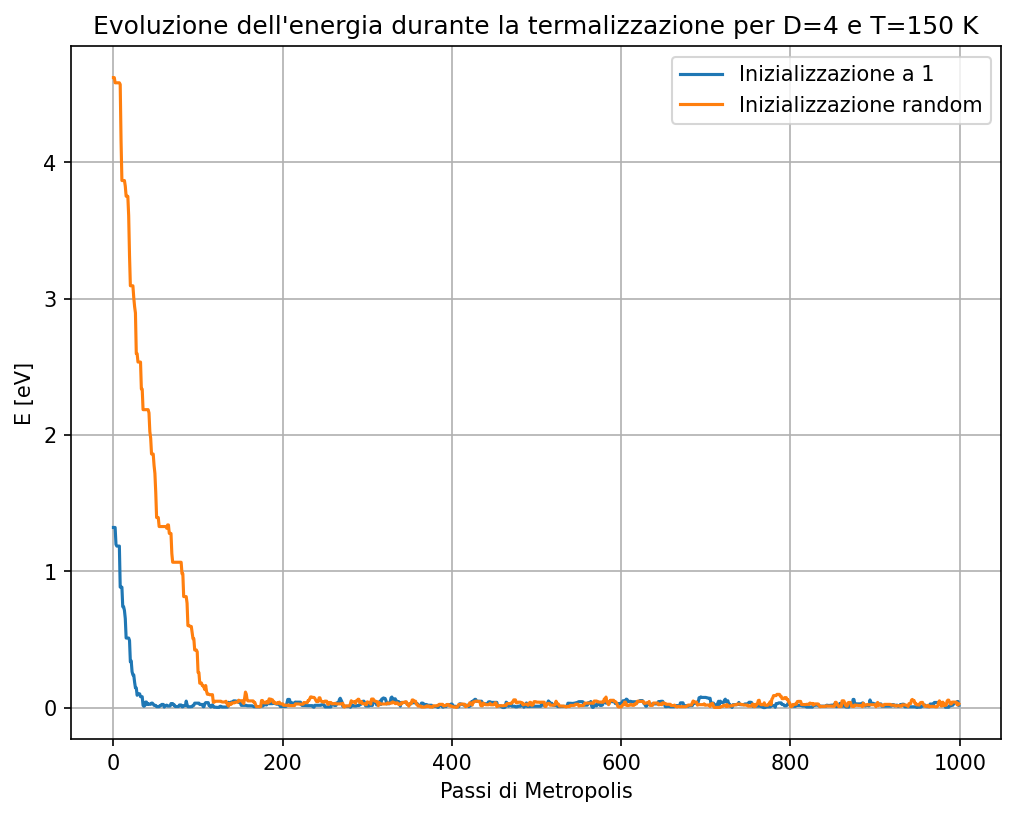
\includegraphics[width=0.9\textwidth]{images/MCMC/thermalization_energies_D4_T150.00.png}
    \caption{}
    \label{fig:therm_T_D}
\end{figure}

\subsection{Risultati}

\begin{figure}[H]
    \centering
    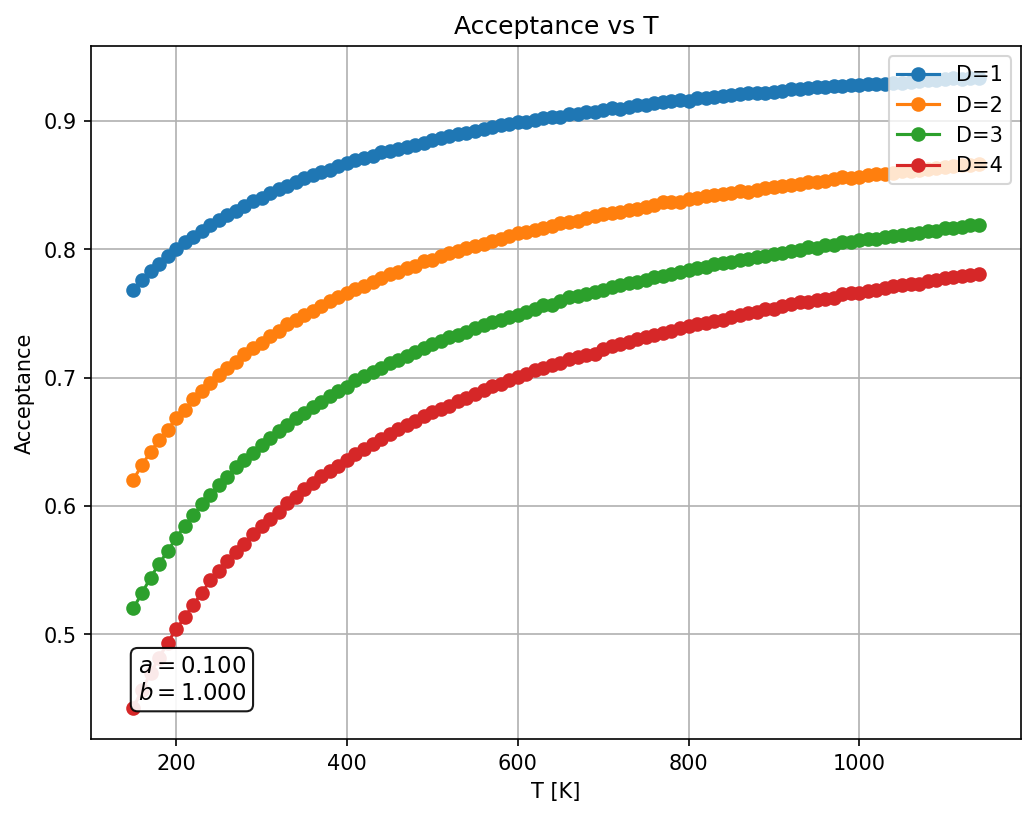
\includegraphics[width=0.9\textwidth]{images/MCMC/acceptance_vs_T.png}
    \caption{}
    \label{fig:acc_T_D}
\end{figure}

\begin{figure}[H]
    \centering
    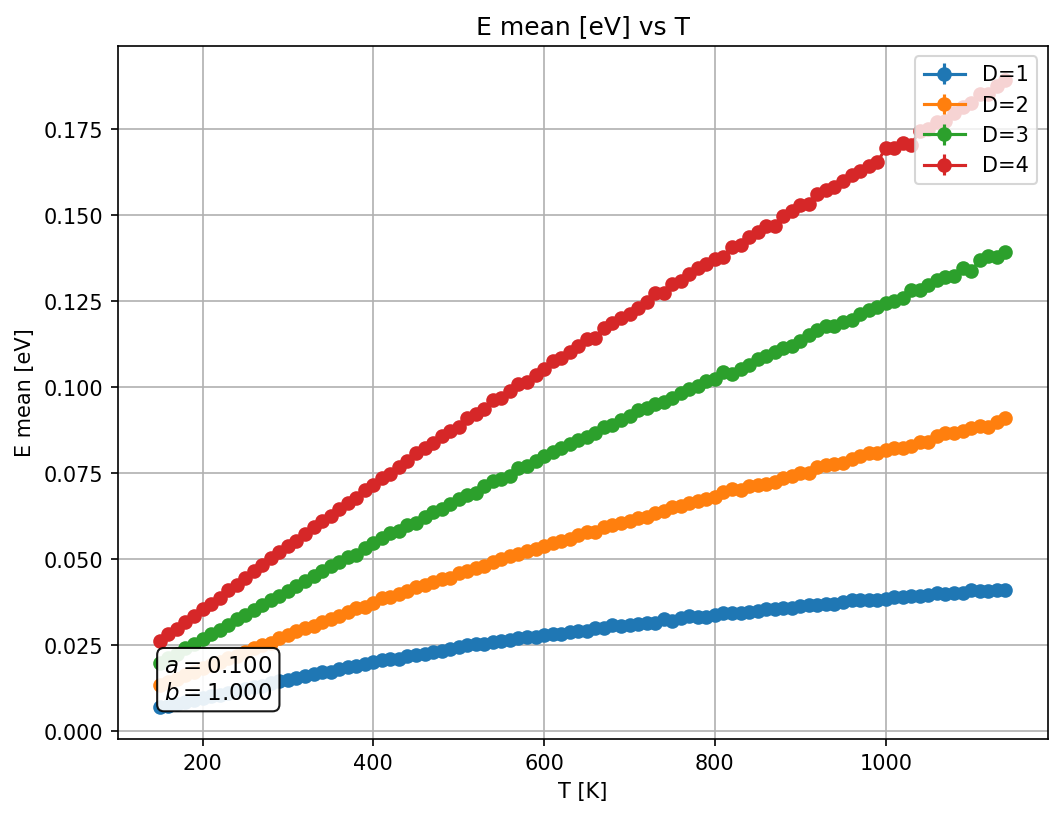
\includegraphics[width=0.9\textwidth]{images/MCMC/E_mean_vs_T.png}
    \caption{}
    \label{fig:E_T_D}
\end{figure}

\begin{figure}[H]
    \centering
    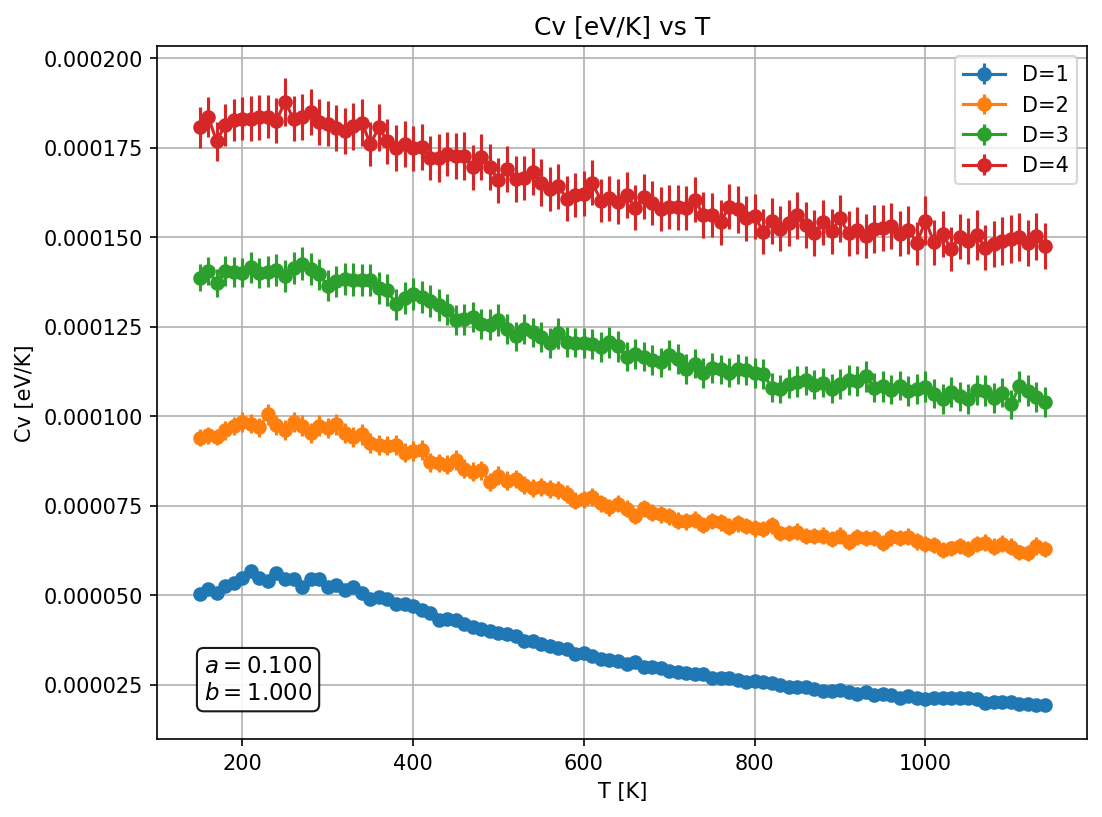
\includegraphics[width=0.9\textwidth]{images/MCMC/Cv_vs_T.png}
    \caption{}
    \label{fig:Cv_T_D}
\end{figure}

\begin{figure}[H]
    \centering
    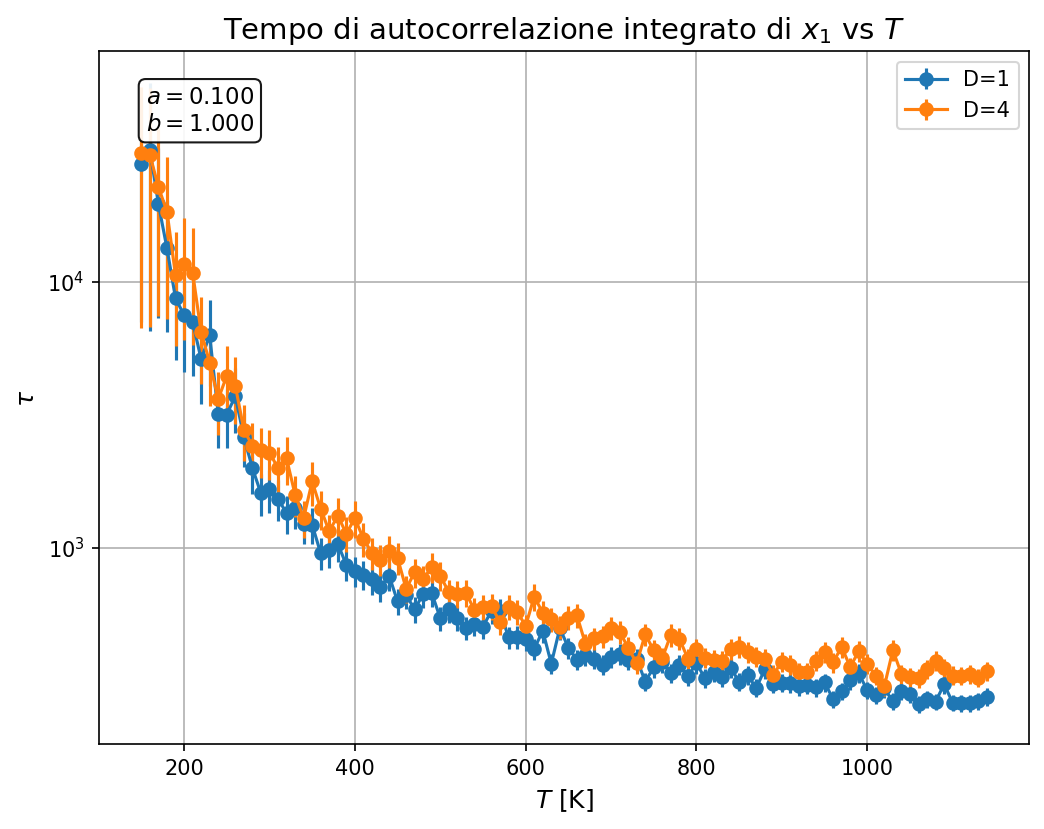
\includegraphics[width=0.9\textwidth]{images/MCMC/Tau_vs_T.png}
    \caption{}
    \label{fig:tau_T_D}
\end{figure}

\section{Confronto dei metodi di campionamento}
\label{sec:confronto_metodi}

\subsection{Dettagli implementativi}

\subsection{Confronto al variare di T}

\begin{figure}[H]
    \centering
    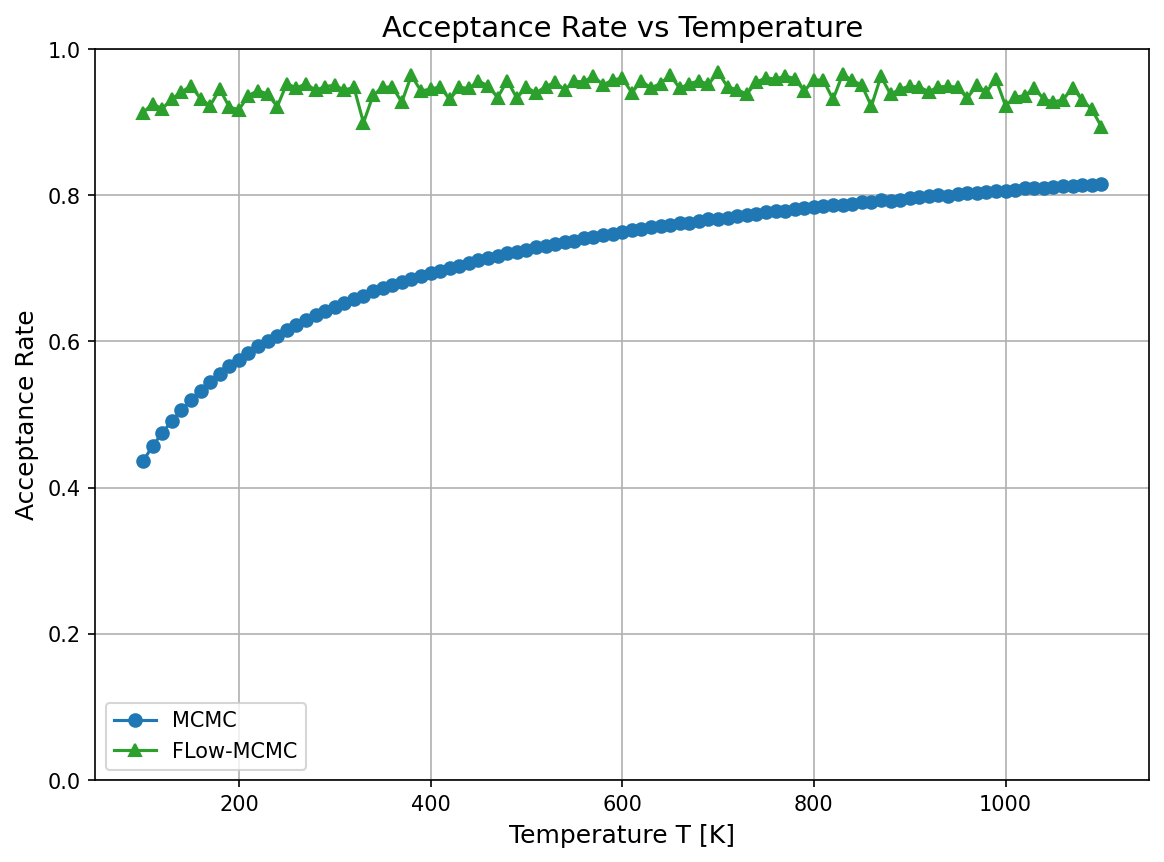
\includegraphics[width=0.9\textwidth]{images/acceptance_vs_T_plot.png}
    \caption{}
    \label{fig:acc_T_all}
\end{figure}

\begin{figure}[H]
    \centering
    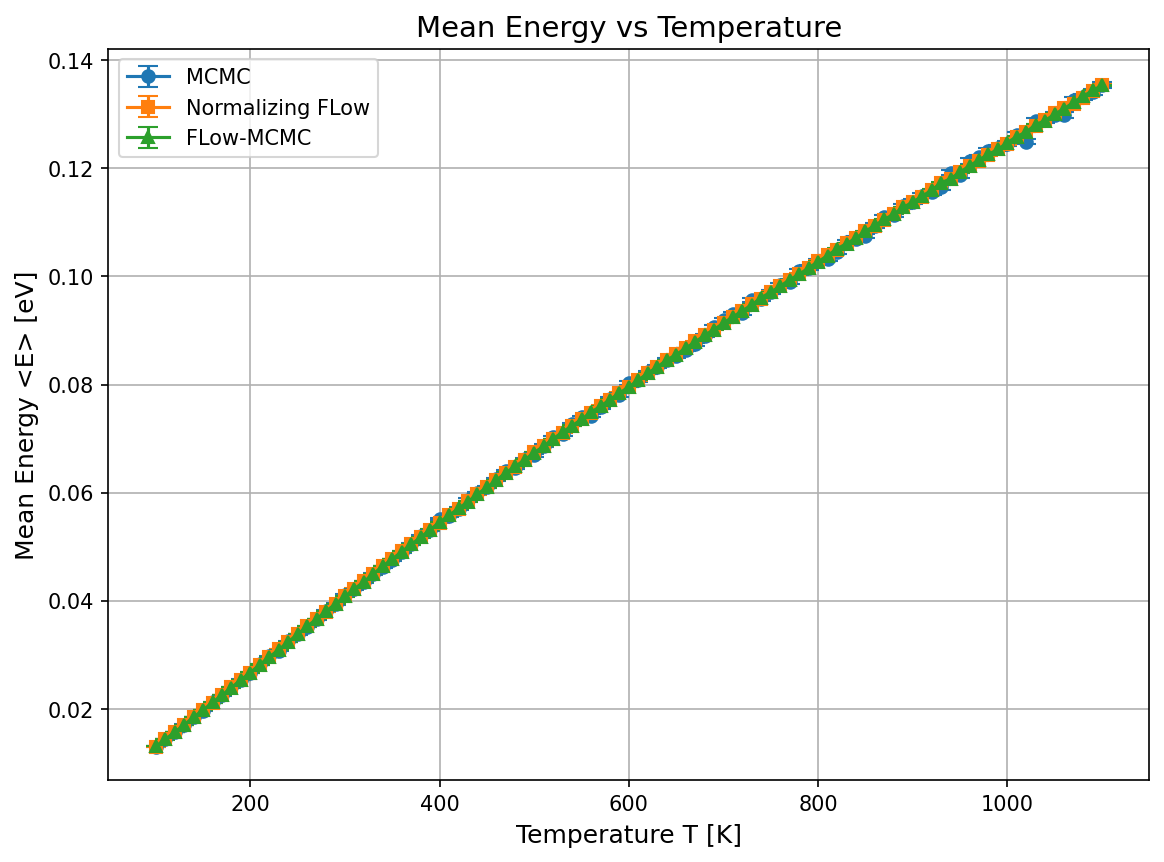
\includegraphics[width=0.9\textwidth]{images/E_vs_T_plot.png}
    \caption{}
    \label{fig:E_T_all}
\end{figure}

\begin{figure}[H]
    \centering
    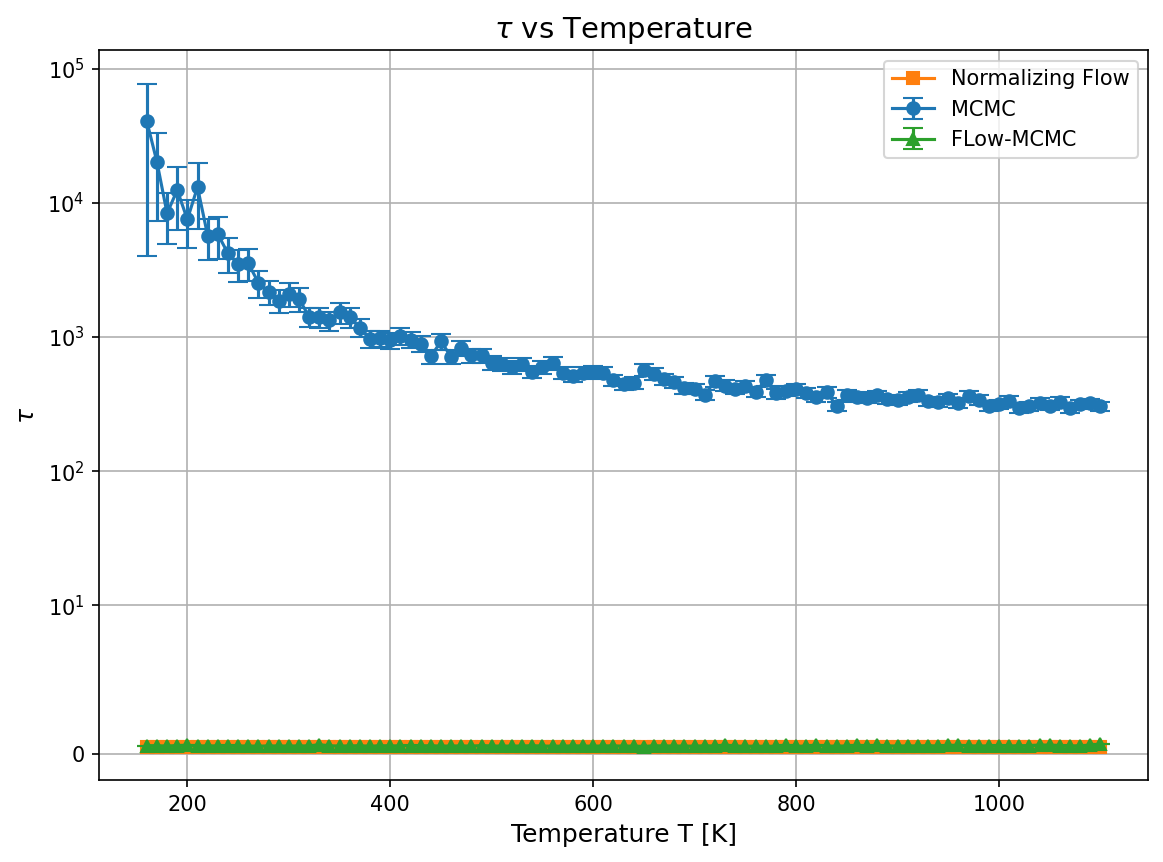
\includegraphics[width=0.9\textwidth]{images/tau_vs_T_plot.png}
    \caption{}
    \label{fig:tau_T_all}
\end{figure}

\begin{figure}[H]
    \centering
    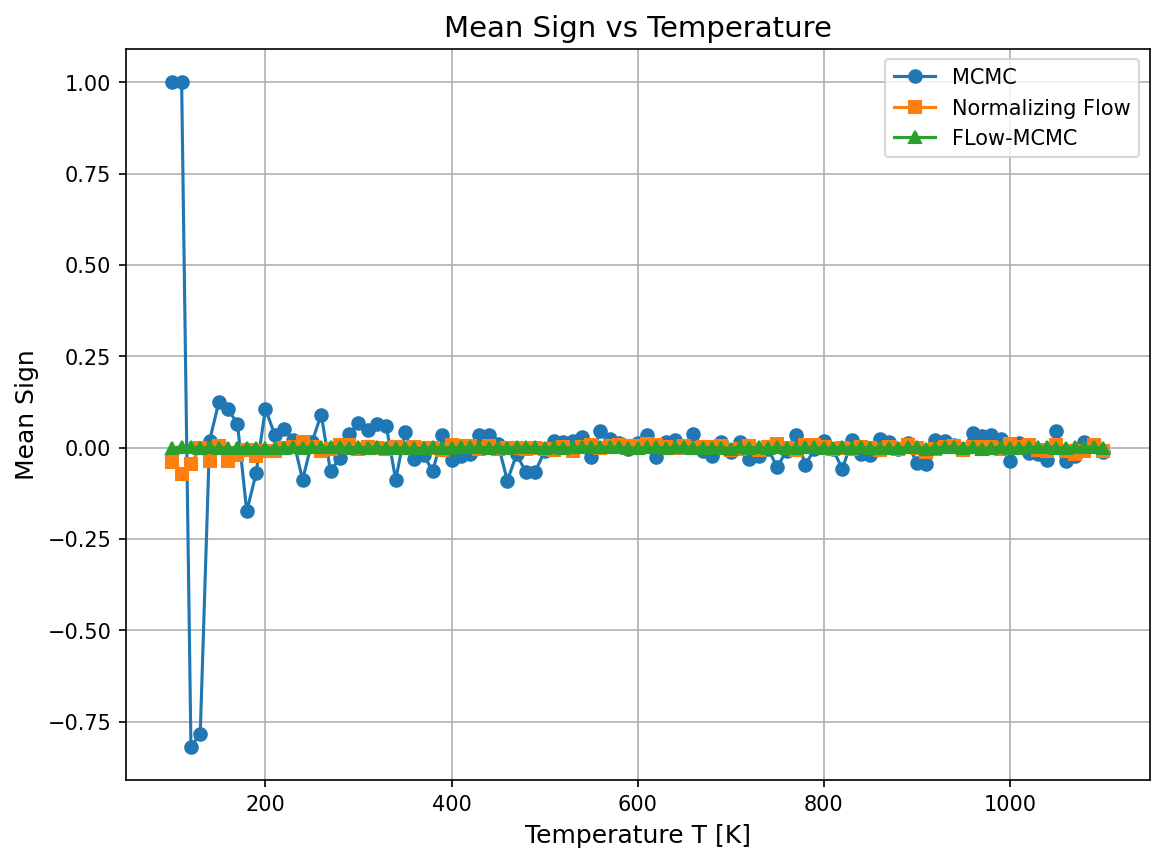
\includegraphics[width=0.9\textwidth]{images/mean_sign_vs_T_plot.png}
    \caption{}
    \label{fig:msig_T_all}
\end{figure}

\subsection{Confronto al variare di N}

\begin{figure}[H]
    \centering
    \begin{subfigure}[b]{0.45\textwidth}
        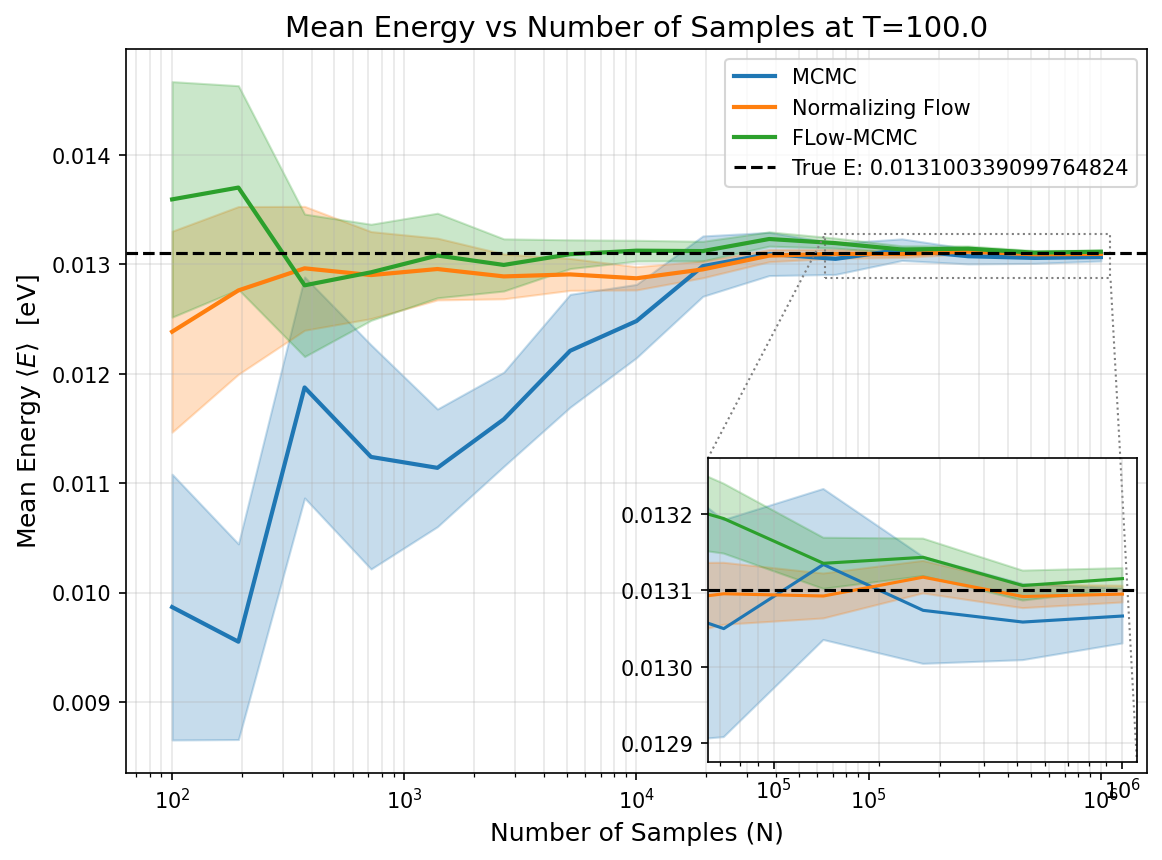
\includegraphics[width=\textwidth]{images/E_vs_N_plot_T_100.0.png}
        \caption{Prima}
    \end{subfigure}
    \hfill
    \begin{subfigure}[b]{0.45\textwidth}
        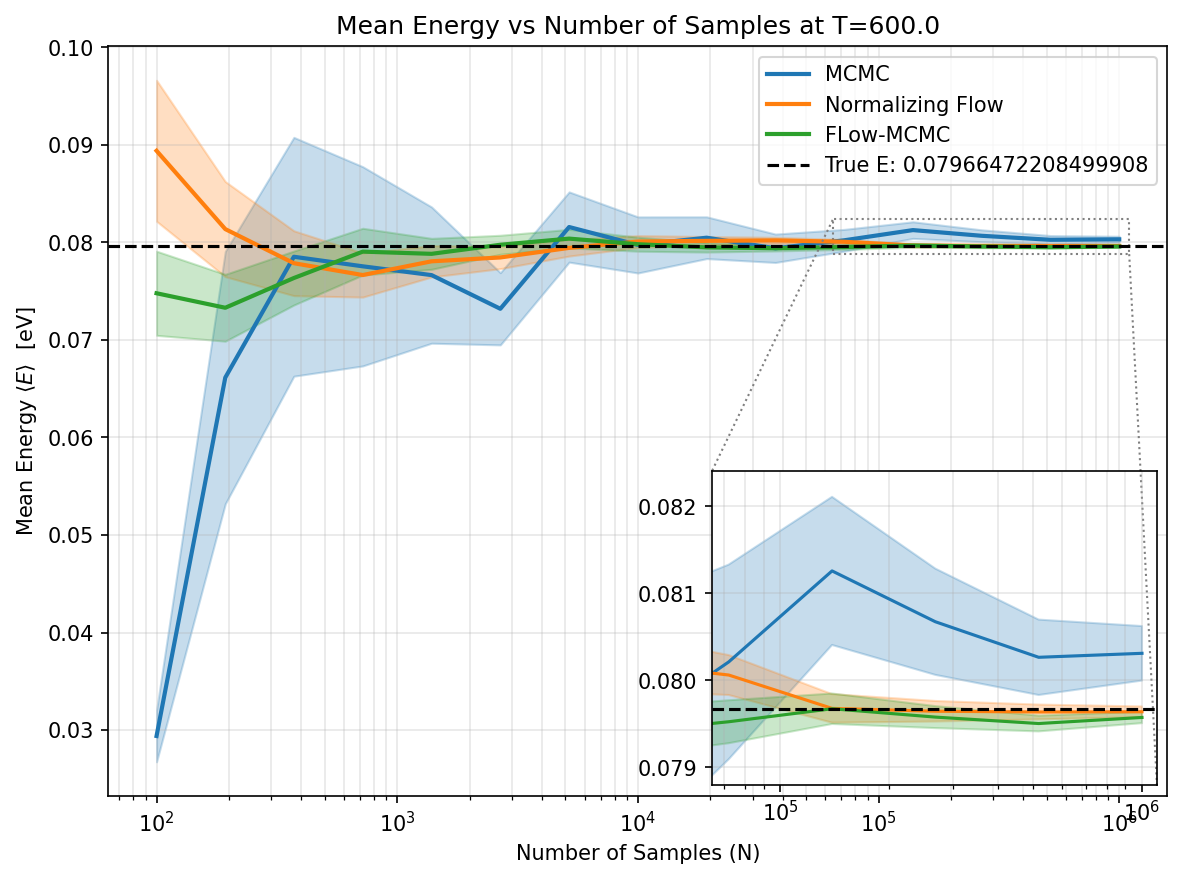
\includegraphics[width=\textwidth]{images/E_vs_N_plot_T_600.0.png}
        \caption{Seconda}
    \end{subfigure}
    
    \vspace{1em}
    
    \begin{subfigure}[b]{0.45\textwidth}
        \centering
        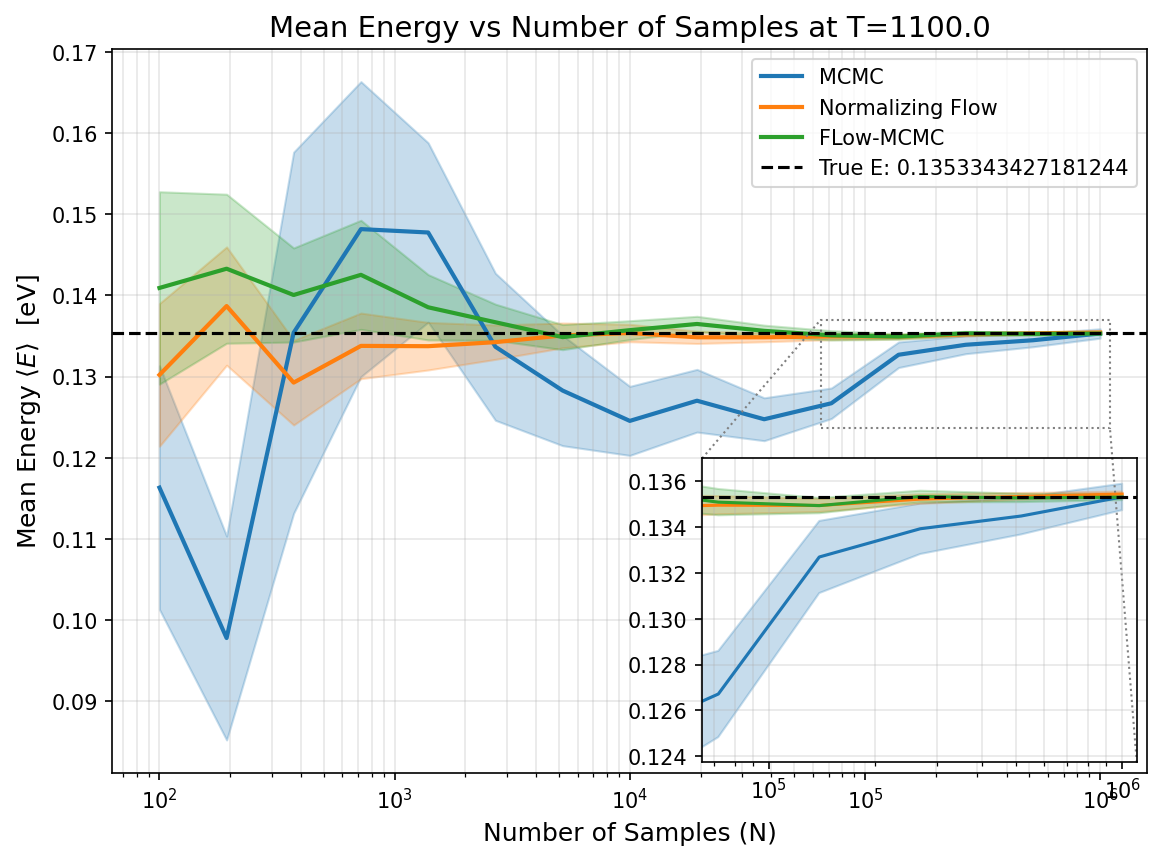
\includegraphics[width=\textwidth]{images/E_vs_N_plot_T_1100.0.png}
        \caption{Terza}
    \end{subfigure}
    \caption{}
\end{figure}

\begin{figure}[H]
    \centering
    \begin{subfigure}[b]{0.45\textwidth}
        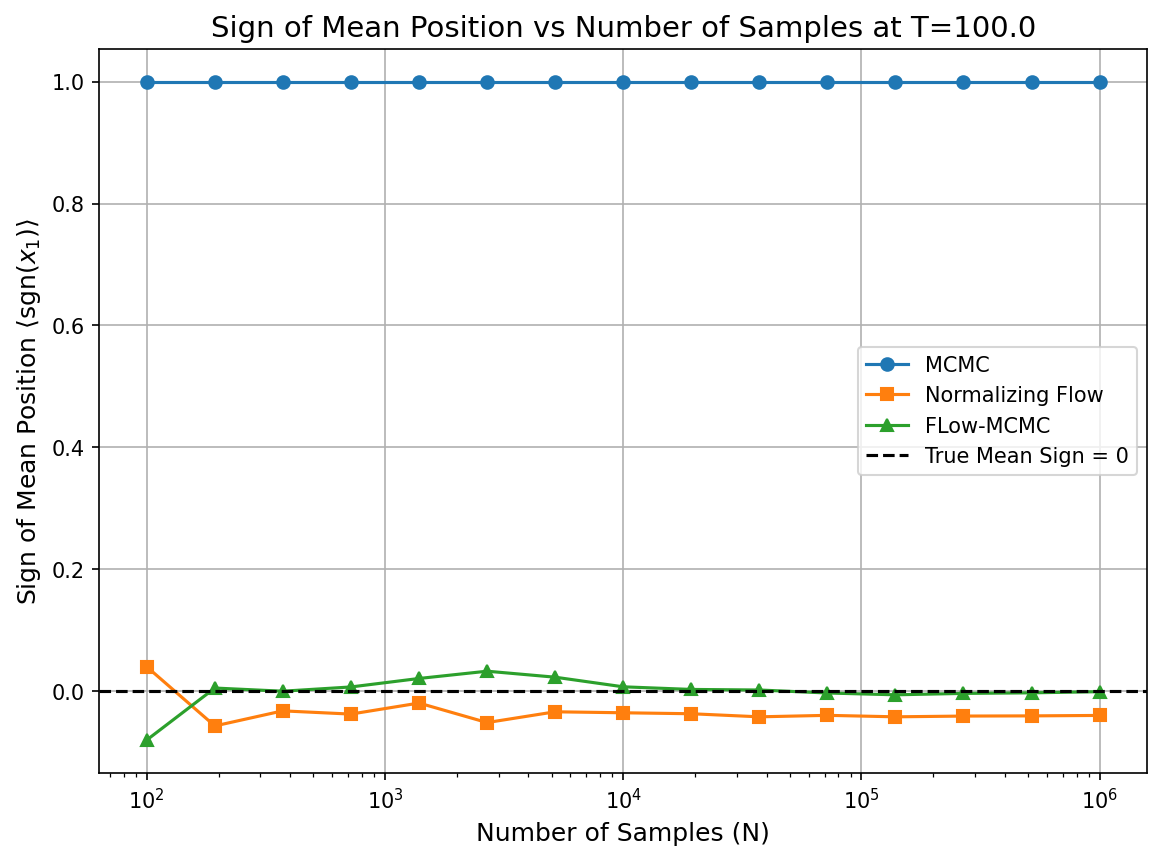
\includegraphics[width=\textwidth]{images/mean_sign_vs_N_plot_T_100.0.png}
        \caption{Prima}
    \end{subfigure}
    \hfill
    \begin{subfigure}[b]{0.45\textwidth}
        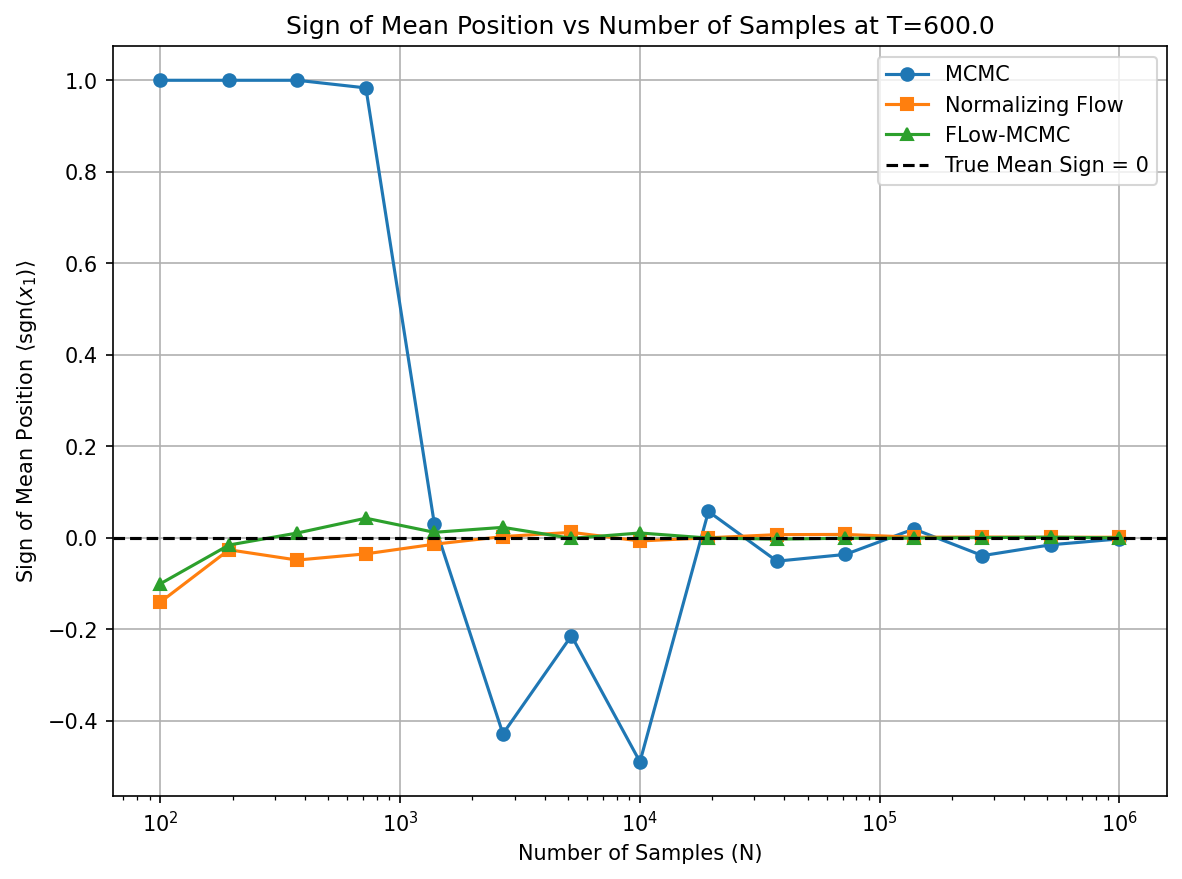
\includegraphics[width=\textwidth]{images/mean_sign_vs_N_plot_T_600.0.png}
        \caption{Seconda}
    \end{subfigure}
    
    \vspace{1em}
    
    \begin{subfigure}[b]{0.45\textwidth}
        \centering
        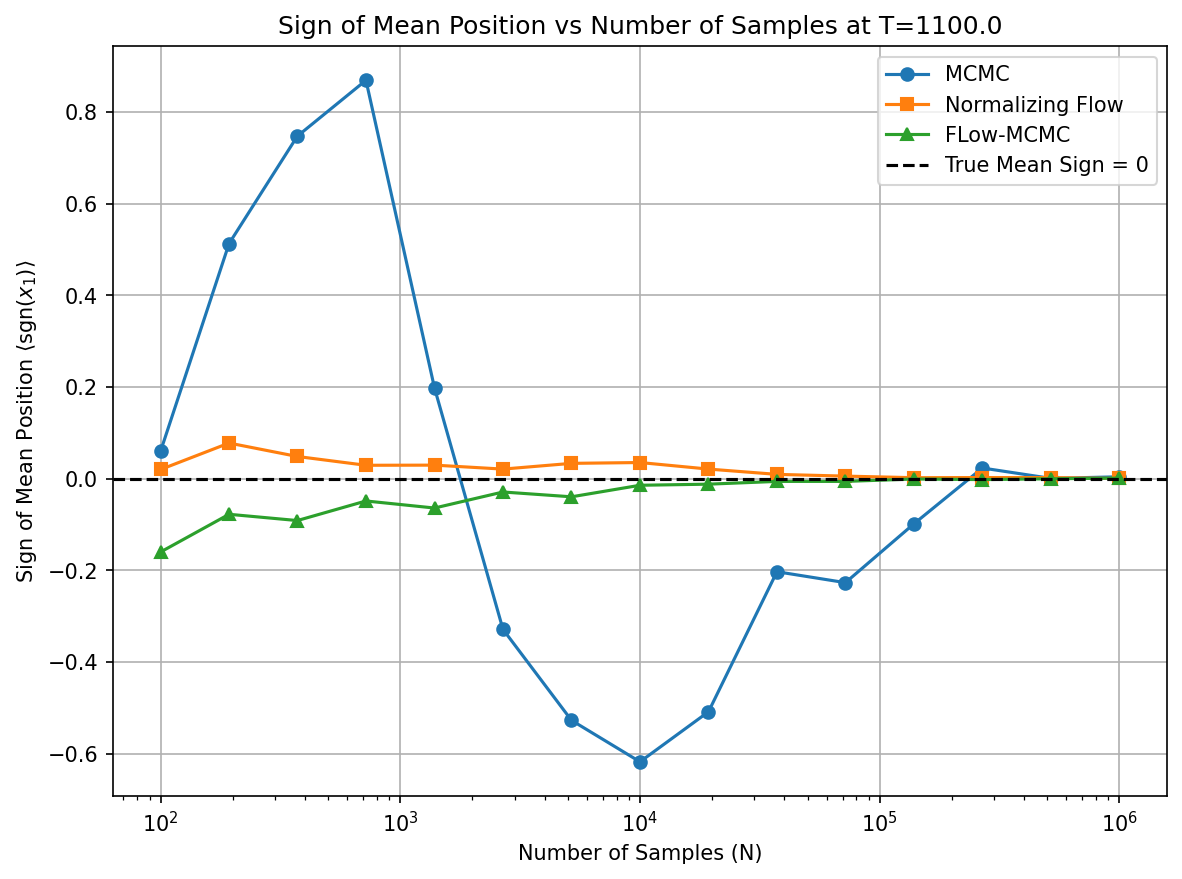
\includegraphics[width=\textwidth]{images/mean_sign_vs_N_plot_T_1100.0.png}
        \caption{Terza}
    \end{subfigure}
    \caption{}
\end{figure}

\subsection{Distribuzioni e traiettorie del camminatore}

\begin{figure}[H]
    \centering
    \begin{subfigure}[b]{0.45\textwidth}
        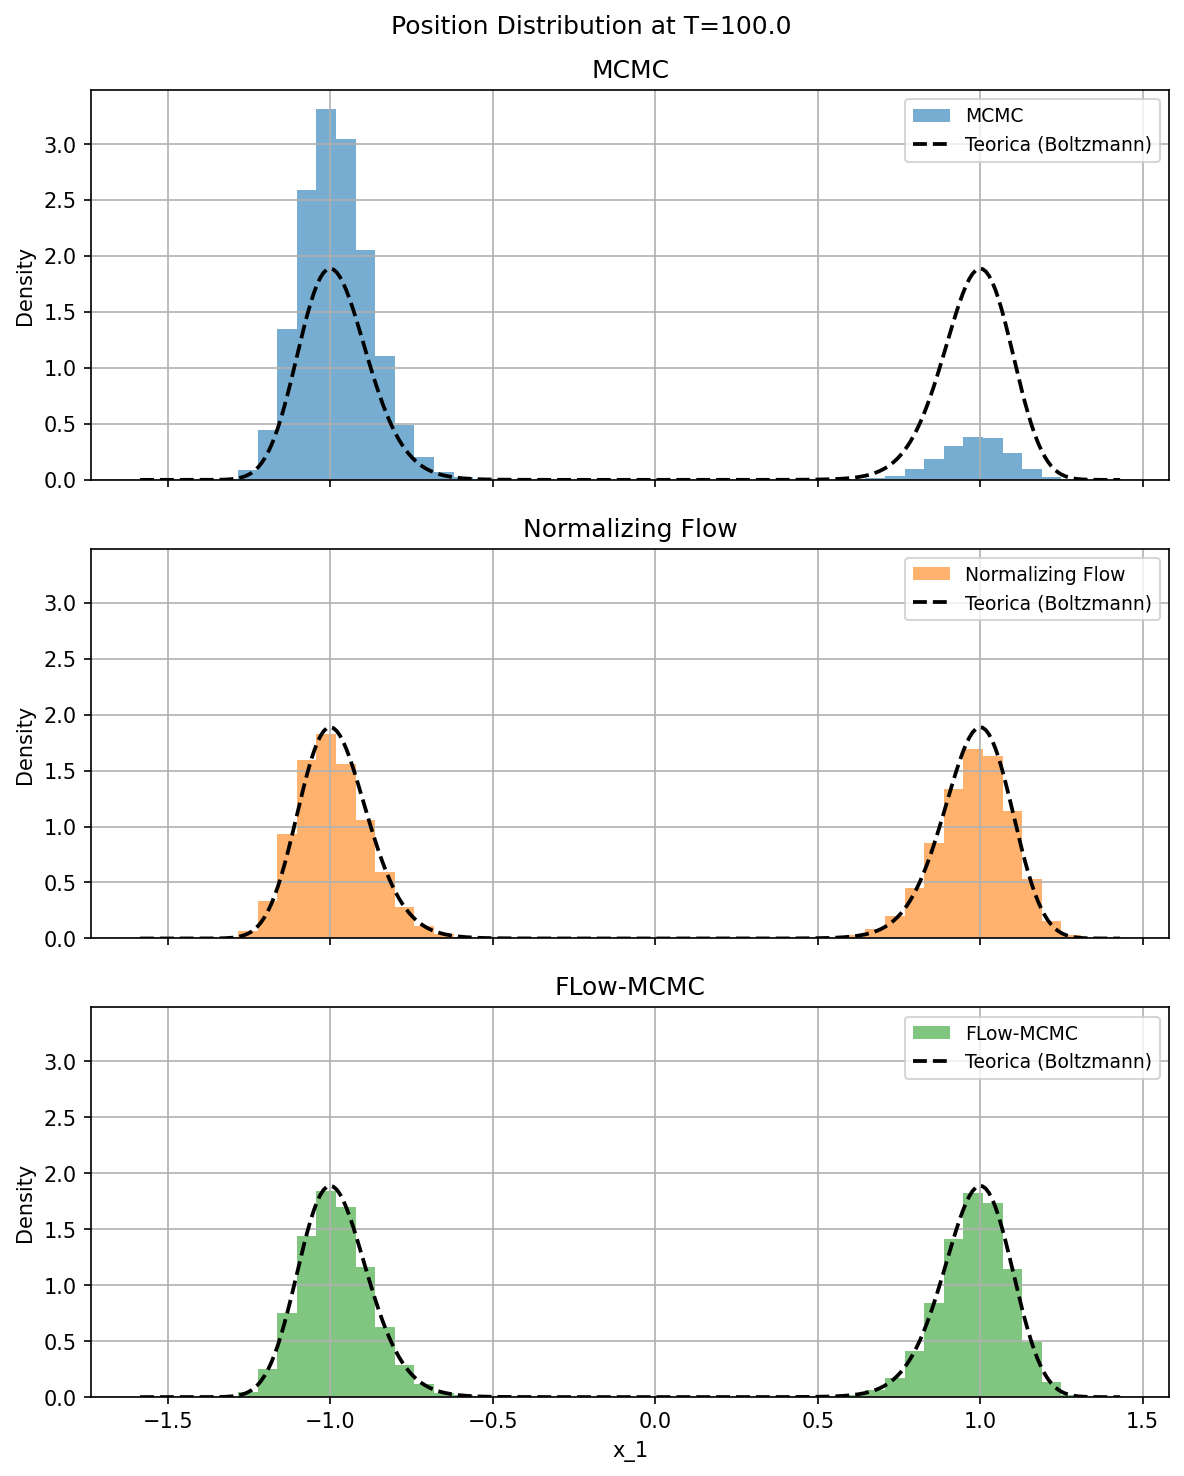
\includegraphics[width=\textwidth]{images/x_distribution_T_100.0.png}
        \caption{Prima}
    \end{subfigure}
    \hfill
    \begin{subfigure}[b]{0.45\textwidth}
        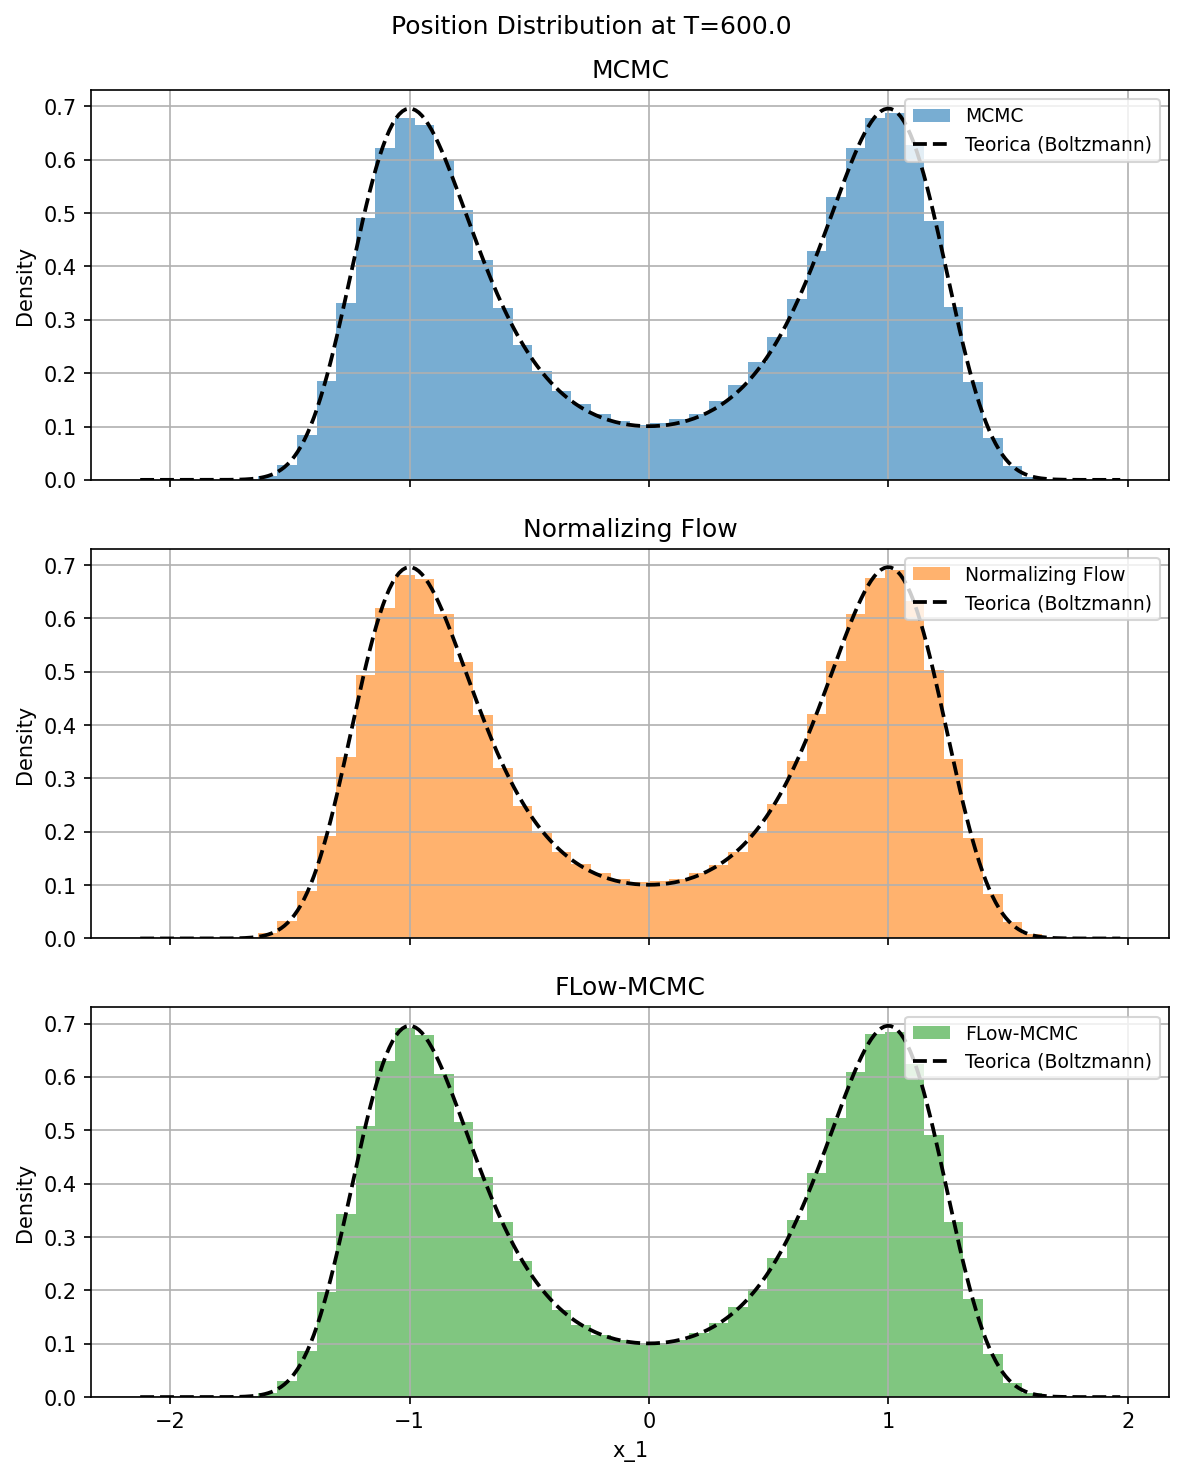
\includegraphics[width=\textwidth]{images/x_distribution_T_600.0.png}
        \caption{Seconda}
    \end{subfigure}
    
    \vspace{1em}
    
    \begin{subfigure}[b]{0.45\textwidth}
        \centering
        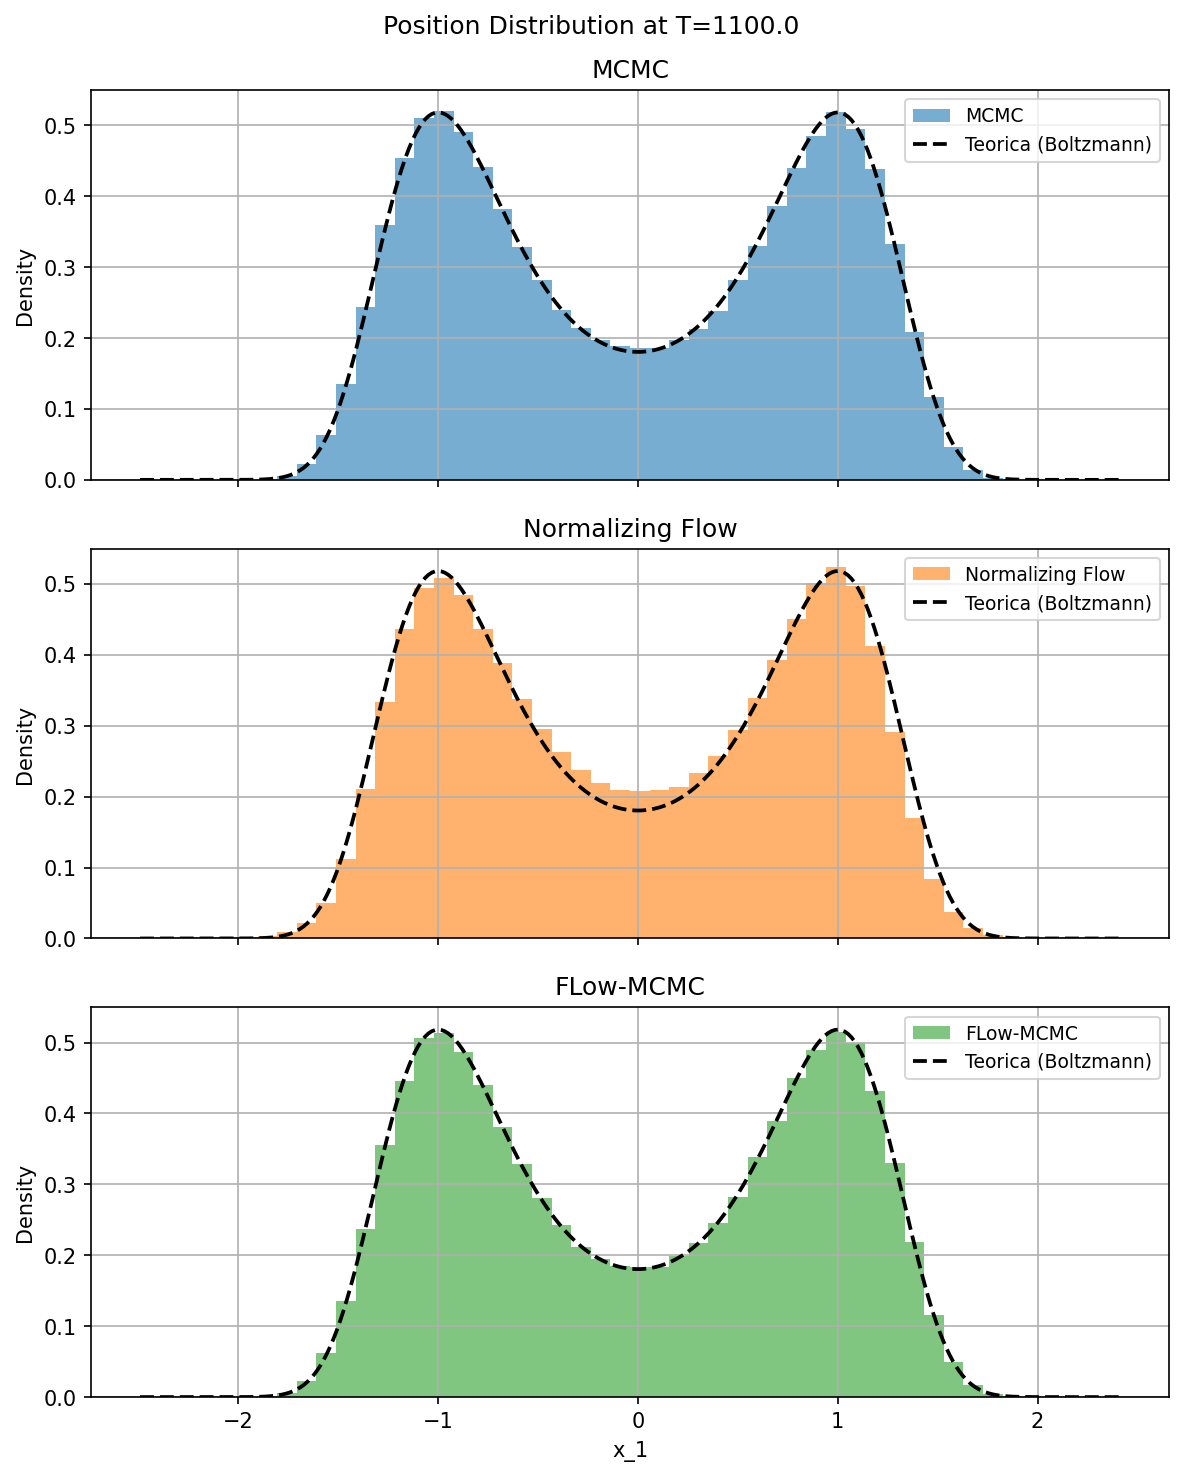
\includegraphics[width=\textwidth]{images/x_distribution_T_1100.0.png}
        \caption{Terza}
    \end{subfigure}
    \caption{}
\end{figure}

\begin{figure}[H]
    \centering
    \begin{subfigure}[b]{0.45\textwidth}
        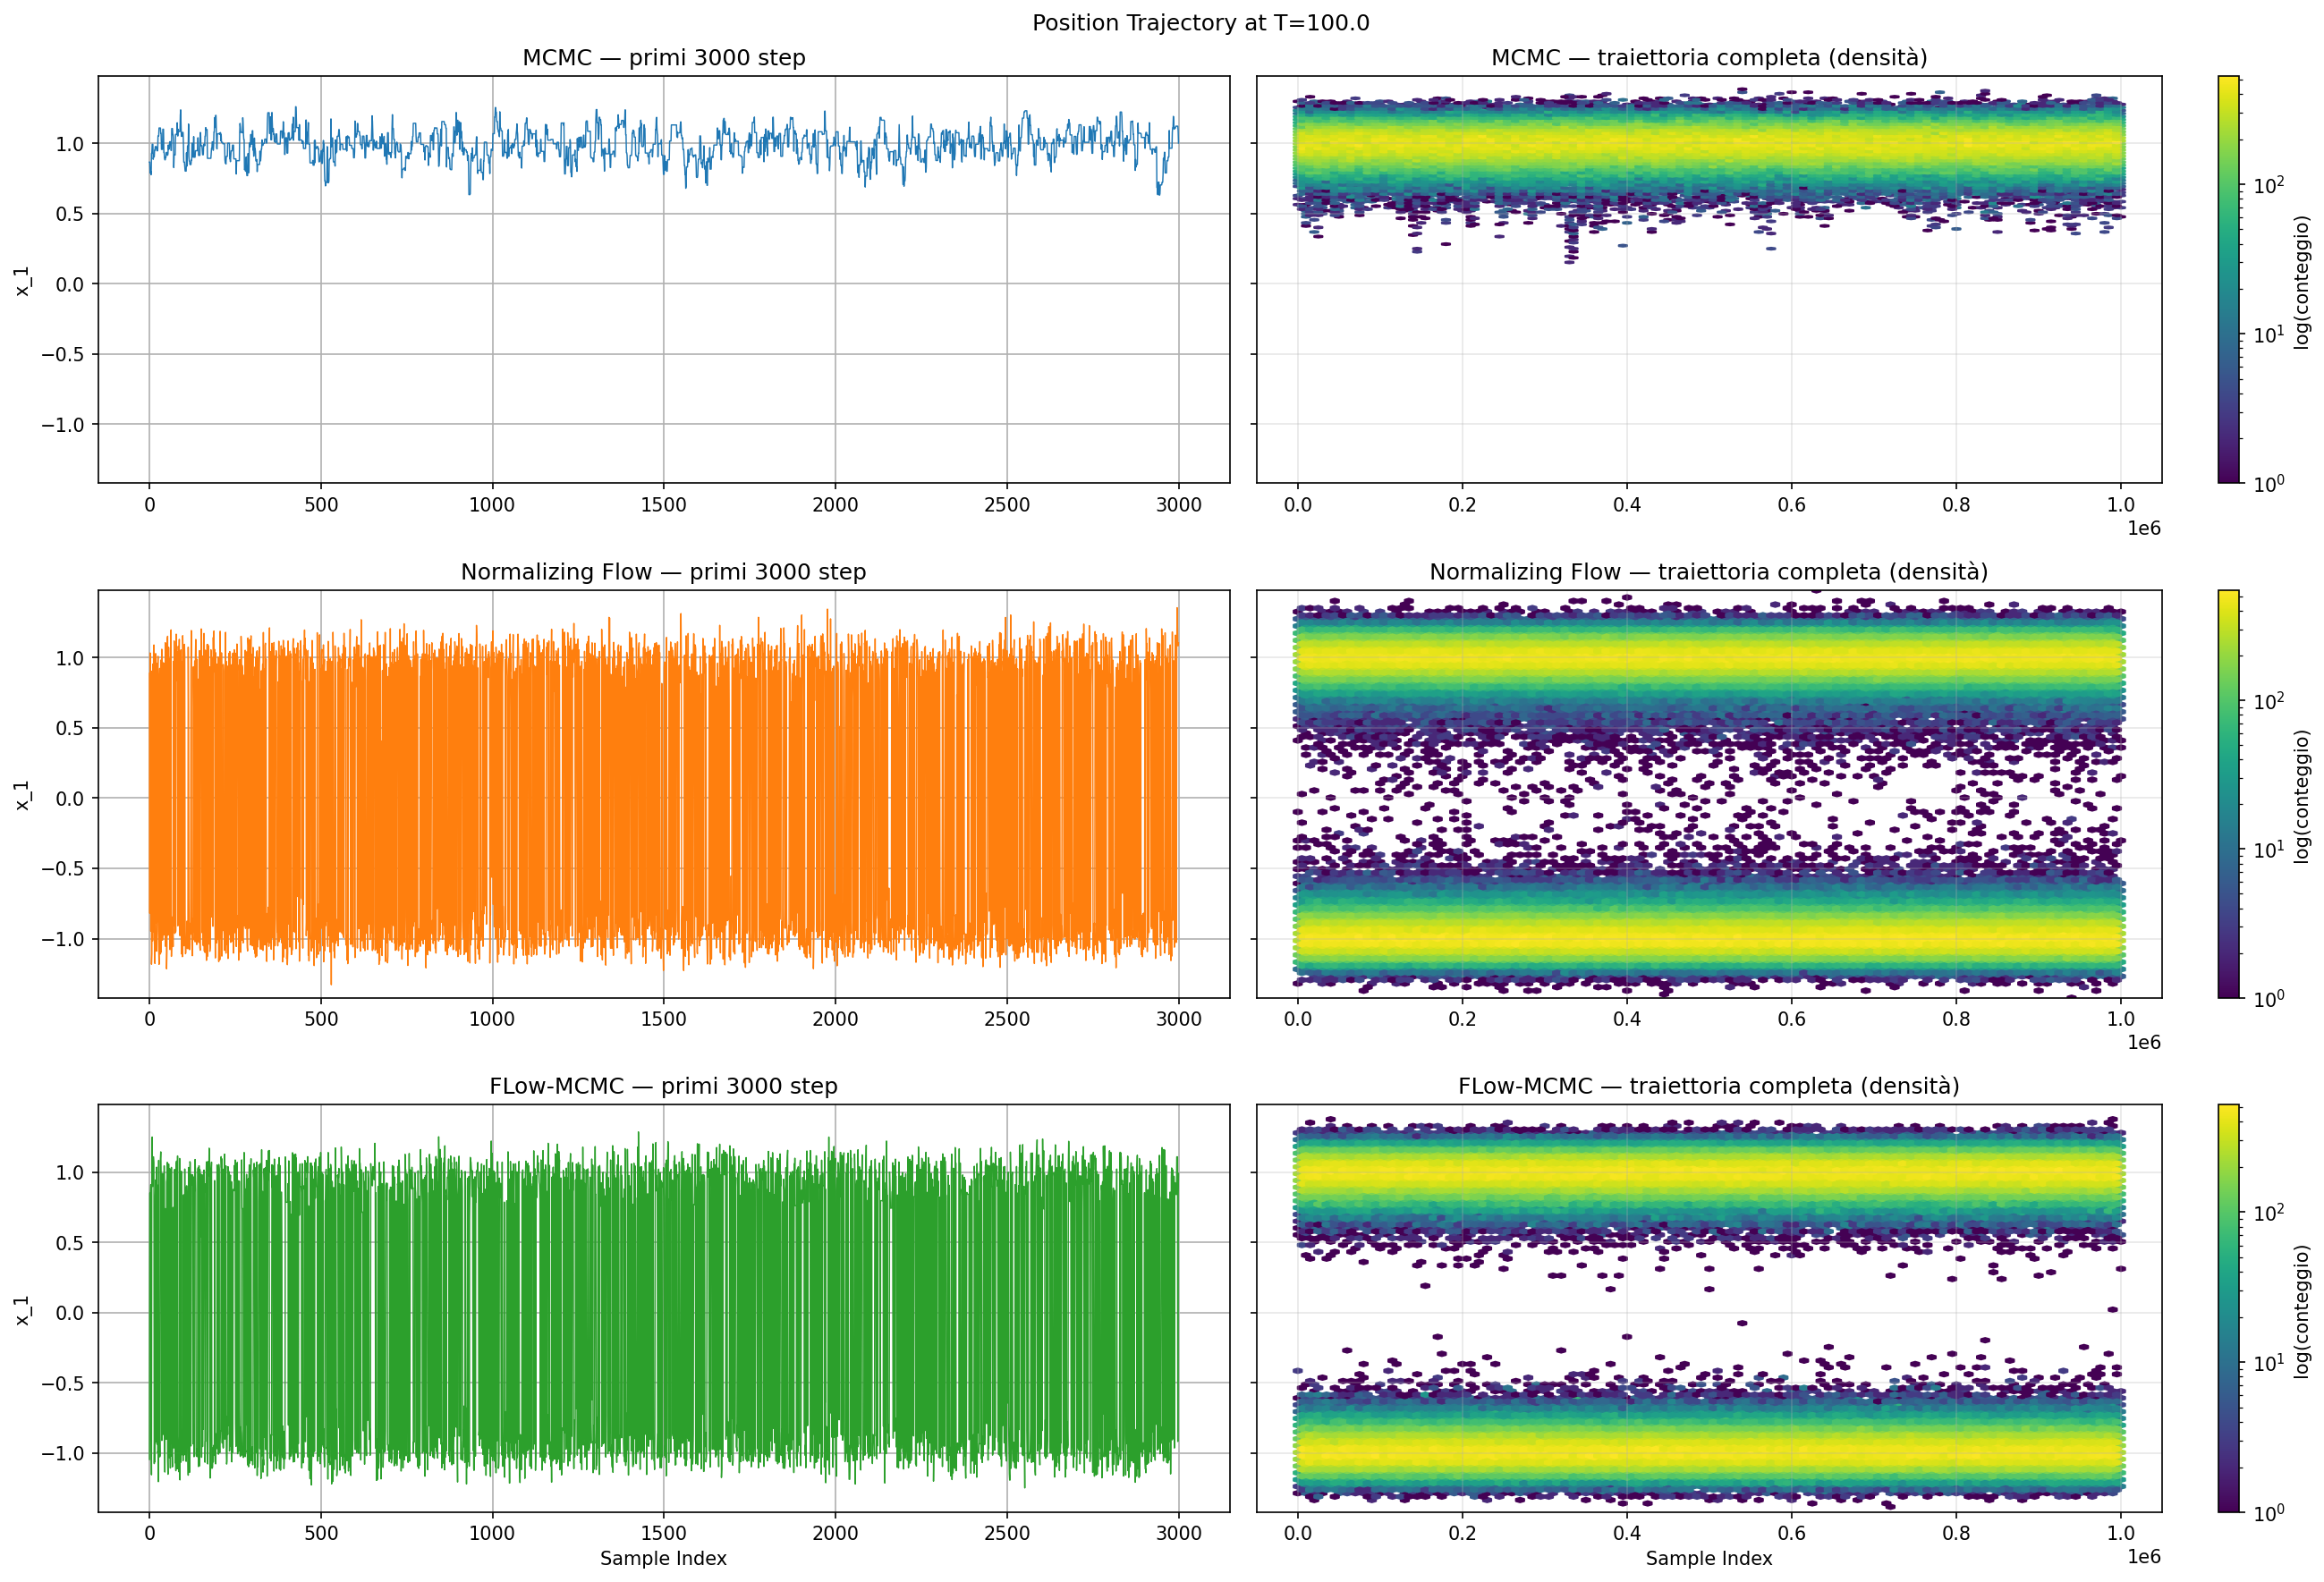
\includegraphics[width=\textwidth]{images/x_trajectory_T_100.0.png}
        \caption{Prima}
    \end{subfigure}
    \hfill
    \begin{subfigure}[b]{0.45\textwidth}
        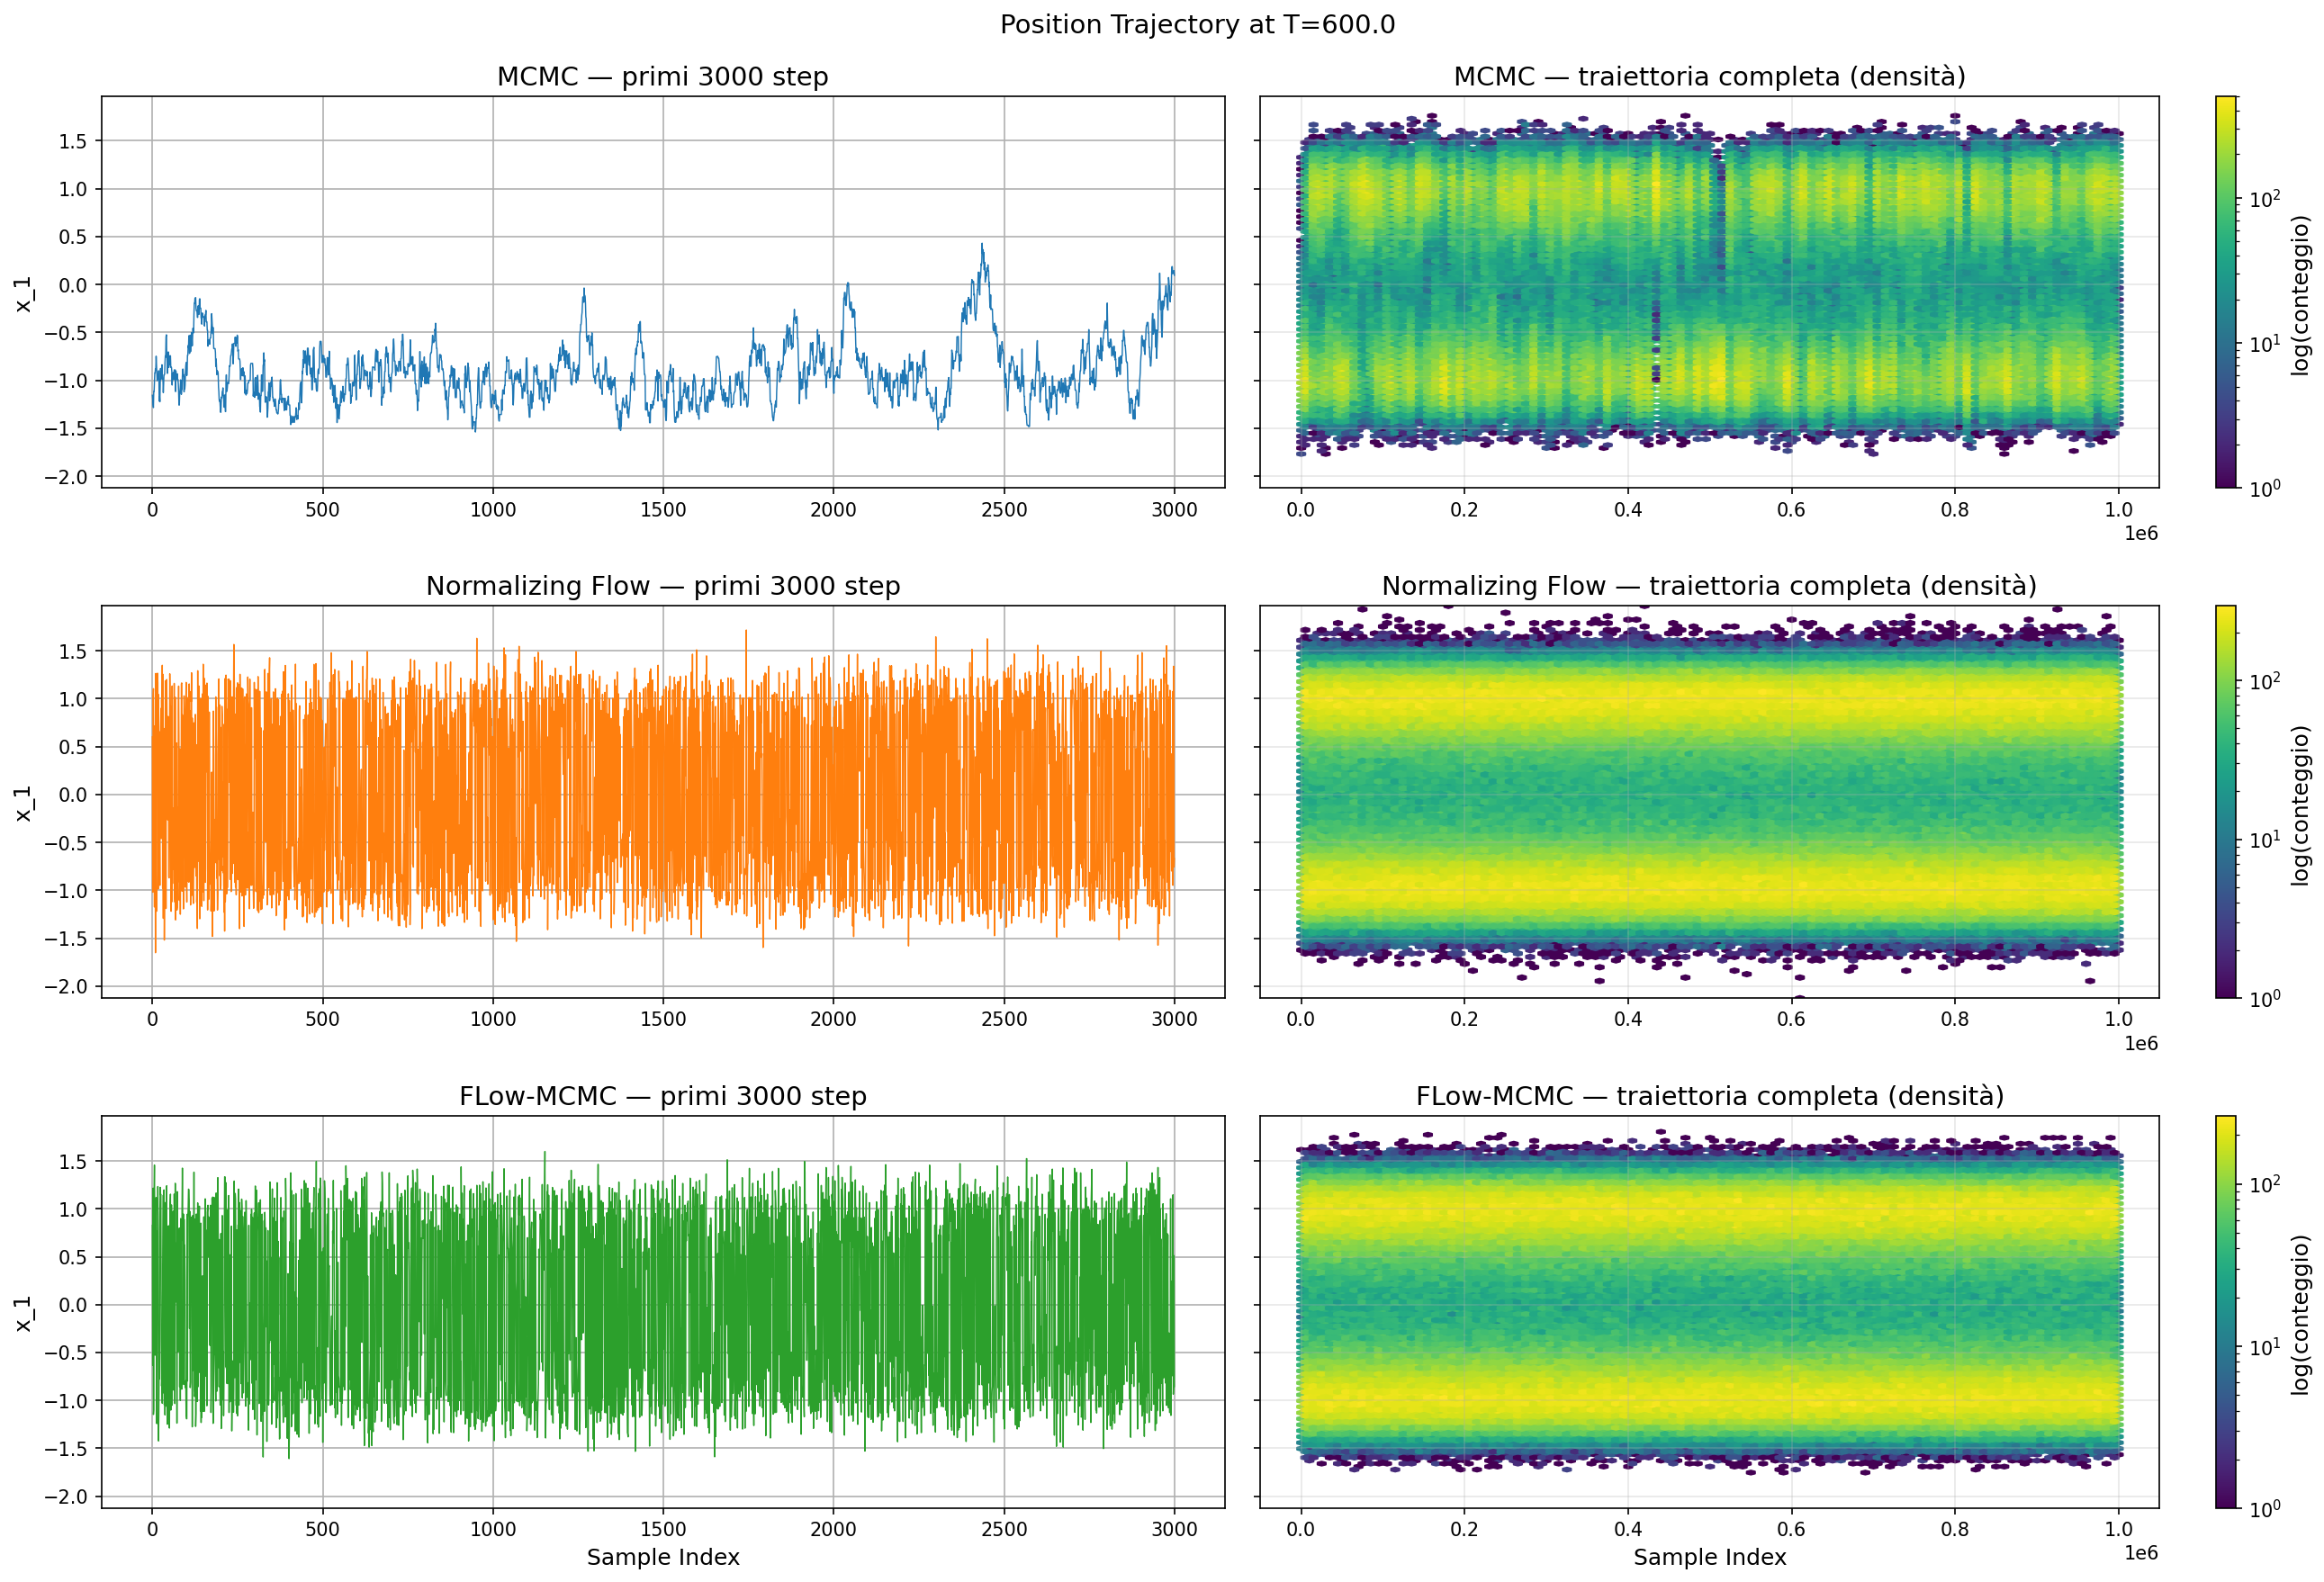
\includegraphics[width=\textwidth]{images/x_trajectory_T_600.0.png}
        \caption{Seconda}
    \end{subfigure}
    
    \vspace{1em}
    
    \begin{subfigure}[b]{0.45\textwidth}
        \centering
        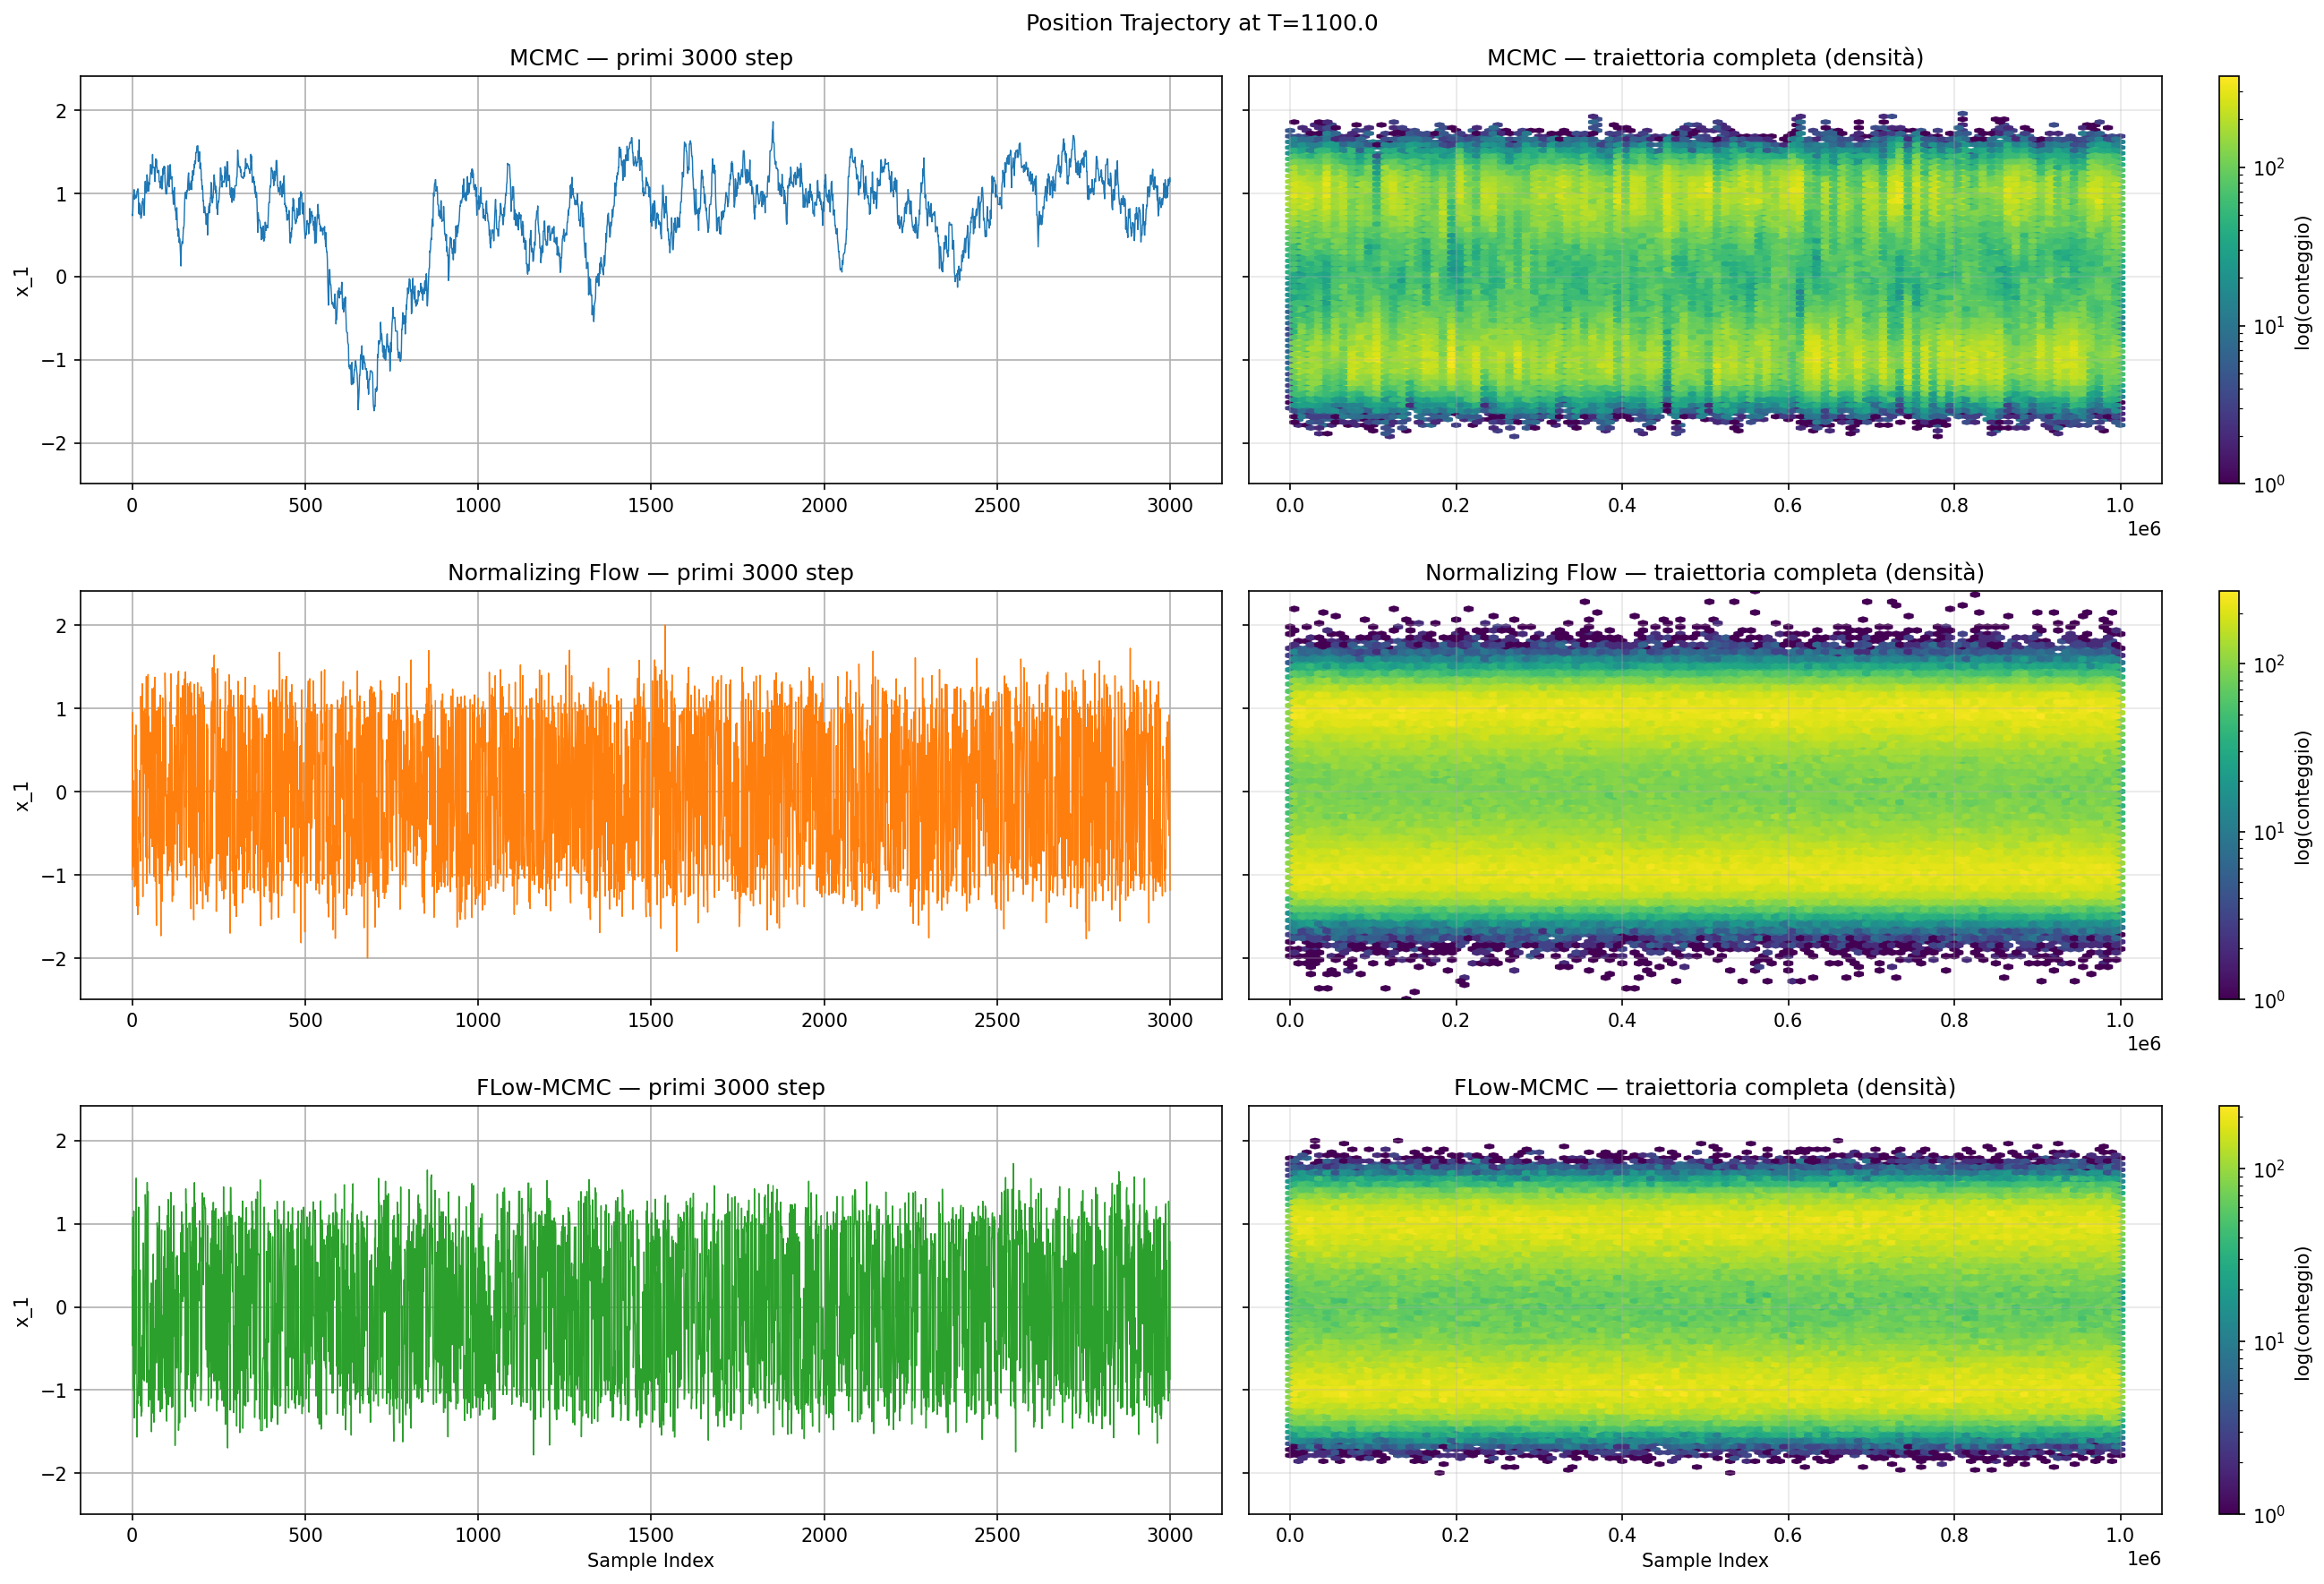
\includegraphics[width=\textwidth]{images/x_trajectory_T_1100.0.png}
        \caption{Terza}
    \end{subfigure}
    \caption{}
\end{figure}

